\section{Results}
\label{sec:res}

We organize our results discussion in three parts: In Section \ref{sec:res_syn}, we compare the performance of our algorithm to that of the benchmark policies on the synthetic dataset with a homogeneous gig worker population. In Section \ref{sec:res_syn_2}, we examine the performance of our algorithm on the synthetic dataset where the gig worker population is heterogeneous, analyzing the impact of correctly modeling multiple gig worker groups versus incorrectly assuming a homogeneous population. Lastly, Section \ref{sec:res_nyt} focuses on the performance of our algorithm using the NYT datasets, for gig workers with weak and strong location preferences. 

\subsection{Homogeneous gig worker population}
\label{sec:res_syn}
We first focus on a simplified case where the gig worker population is homogeneous, represented by a single group (D = 1). We examine three sub-scenarios (I.1–I.3), each with different arrival rates of on-demand requests. The benchmarks include the \gls{acr:pp}, \gls{acr:fp}, and Pert. ($\epsilon=0$), alongside our algorithm, employing a single \gls{acr:mnl} model in alignment with the environmental conditions. 

\begin{figure}[t]%
    \centering
    \fontsize{9}{9}\selectfont
    \subfloat[\footnotesize \centering Scen. I.1: Equal arrival rates]{{\adjustbox{width=0.32\textwidth}{% This file was created with tikzplotlib v0.10.1.
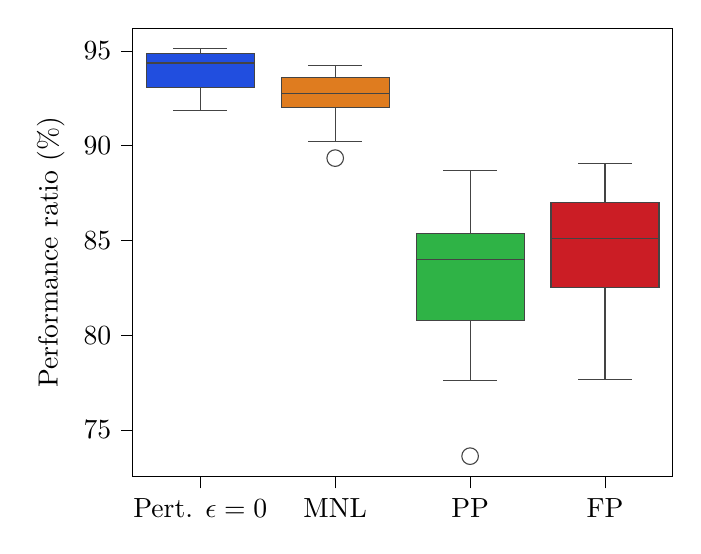
\begin{tikzpicture}

\definecolor{chocolate22312431}{RGB}{223,124,31}
\definecolor{darkgray176}{RGB}{176,176,176}
\definecolor{darkslategray68}{RGB}{68,68,68}
\definecolor{firebrick2032937}{RGB}{203,29,37}
\definecolor{limegreen4717970}{RGB}{47,179,70}
\definecolor{royalblue3378223}{RGB}{33,78,223}

\begin{axis}[
tick align=outside,
tick pos=left,
x grid style={darkgray176},
xmin=-0.5, xmax=3.5,
xtick style={color=black},
xtick={0,1,2,3},
xticklabels={Pert. \(\displaystyle \epsilon=0\),MNL,PP,FP},
y grid style={darkgray176},
ylabel={Performance ratio (\%)},
ymin=72.5467977566071, ymax=96.2003769214691,
ytick style={color=black},
ytick={70,75,80,85,90,95,100},
yticklabels={
  \(\displaystyle {70}\),
  \(\displaystyle {75}\),
  \(\displaystyle {80}\),
  \(\displaystyle {85}\),
  \(\displaystyle {90}\),
  \(\displaystyle {95}\),
  \(\displaystyle {100}\)
}
]
\path [draw=darkslategray68, fill=royalblue3378223]
(axis cs:-0.4,93.0765634615927)
--(axis cs:0.4,93.0765634615927)
--(axis cs:0.4,94.8837217605645)
--(axis cs:-0.4,94.8837217605645)
--(axis cs:-0.4,93.0765634615927)
--cycle;
\addplot [darkslategray68]
table {%
0 93.0765634615927
0 91.8523982442826
};
\addplot [darkslategray68]
table {%
0 94.8837217605645
0 95.1252142321572
};
\addplot [darkslategray68]
table {%
-0.2 91.8523982442826
0.2 91.8523982442826
};
\addplot [darkslategray68]
table {%
-0.2 95.1252142321572
0.2 95.1252142321572
};
\path [draw=darkslategray68, fill=chocolate22312431]
(axis cs:0.6,92.0224894960145)
--(axis cs:1.4,92.0224894960145)
--(axis cs:1.4,93.6162686656397)
--(axis cs:0.6,93.6162686656397)
--(axis cs:0.6,92.0224894960145)
--cycle;
\addplot [darkslategray68]
table {%
1 92.0224894960145
1 90.2346005578498
};
\addplot [darkslategray68]
table {%
1 93.6162686656397
1 94.2259197773107
};
\addplot [darkslategray68]
table {%
0.8 90.2346005578498
1.2 90.2346005578498
};
\addplot [darkslategray68]
table {%
0.8 94.2259197773107
1.2 94.2259197773107
};
\addplot [black, mark=o, mark size=3, mark options={solid,fill opacity=0,draw=darkslategray68}, only marks]
table {%
1 89.347001997502
};
\path [draw=darkslategray68, fill=limegreen4717970]
(axis cs:1.6,80.7656222923379)
--(axis cs:2.4,80.7656222923379)
--(axis cs:2.4,85.3874874430389)
--(axis cs:1.6,85.3874874430389)
--(axis cs:1.6,80.7656222923379)
--cycle;
\addplot [darkslategray68]
table {%
2 80.7656222923379
2 77.6341964522543
};
\addplot [darkslategray68]
table {%
2 85.3874874430389
2 88.7043764630758
};
\addplot [darkslategray68]
table {%
1.8 77.6341964522543
2.2 77.6341964522543
};
\addplot [darkslategray68]
table {%
1.8 88.7043764630758
2.2 88.7043764630758
};
\addplot [black, mark=o, mark size=3, mark options={solid,fill opacity=0,draw=darkslategray68}, only marks]
table {%
2 73.621960445919
};
\path [draw=darkslategray68, fill=firebrick2032937]
(axis cs:2.6,82.5021621714283)
--(axis cs:3.4,82.5021621714283)
--(axis cs:3.4,87.0227157031759)
--(axis cs:2.6,87.0227157031759)
--(axis cs:2.6,82.5021621714283)
--cycle;
\addplot [darkslategray68]
table {%
3 82.5021621714283
3 77.6603881814643
};
\addplot [darkslategray68]
table {%
3 87.0227157031759
3 89.0406873356241
};
\addplot [darkslategray68]
table {%
2.8 77.6603881814643
3.2 77.6603881814643
};
\addplot [darkslategray68]
table {%
2.8 89.0406873356241
3.2 89.0406873356241
};
\addplot [darkslategray68]
table {%
-0.4 94.3656415323535
0.4 94.3656415323535
};
\addplot [darkslategray68]
table {%
0.6 92.7418460931945
1.4 92.7418460931945
};
\addplot [darkslategray68]
table {%
1.6 84.0058825970647
2.4 84.0058825970647
};
\addplot [darkslategray68]
table {%
2.6 85.0975996089361
3.4 85.0975996089361
};
\draw (axis cs:0,66.6334029653916) node[
  scale=0.75,
  anchor=base,
  text=black,
  rotate=0.0
]{\bfseries 94.00};
\draw (axis cs:1,66.6334029653916) node[
  scale=0.75,
  anchor=base,
  text=black,
  rotate=0.0
]{\bfseries 92.61};
\draw (axis cs:2,66.6334029653916) node[
  scale=0.75,
  anchor=base,
  text=black,
  rotate=0.0
]{\bfseries 83.05};
\draw (axis cs:3,66.6334029653916) node[
  scale=0.75,
  anchor=base,
  text=black,
  rotate=0.0
]{\bfseries 84.65};
\draw (axis cs:-1,66.8699387570403) node[
  scale=0.75,
  text=black,
  rotate=0.0
]{\bfseries \textbf{Average:}};
\end{axis}

\end{tikzpicture}
} }}%
    \hspace*{0.1cm} 
    \subfloat[\footnotesize \centering Scen. I.2: Lower request arrival rate]{{\adjustbox{width=0.32\textwidth}{% This file was created with tikzplotlib v0.10.1.
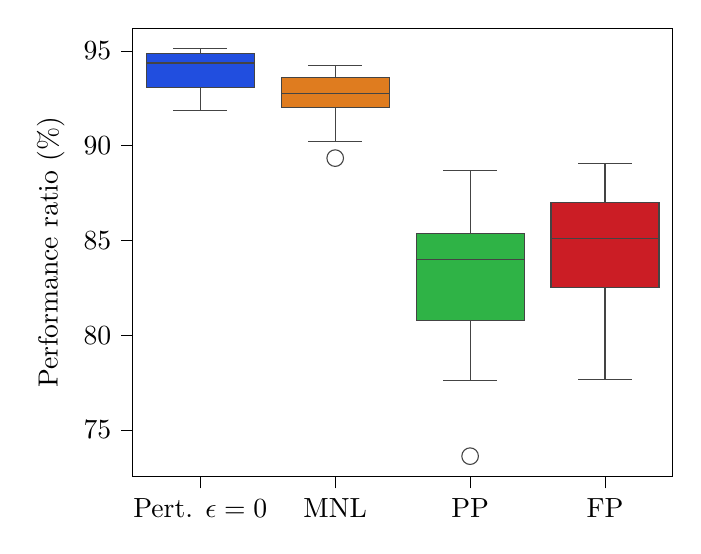
\begin{tikzpicture}

\definecolor{chocolate22312431}{RGB}{223,124,31}
\definecolor{darkgray176}{RGB}{176,176,176}
\definecolor{darkslategray68}{RGB}{68,68,68}
\definecolor{firebrick2032937}{RGB}{203,29,37}
\definecolor{limegreen4717970}{RGB}{47,179,70}
\definecolor{royalblue3378223}{RGB}{33,78,223}

\begin{axis}[
tick align=outside,
tick pos=left,
x grid style={darkgray176},
xmin=-0.5, xmax=3.5,
xtick style={color=black},
xtick={0,1,2,3},
xticklabels={Pert. \(\displaystyle \epsilon=0\),MNL,PP,FP},
y grid style={darkgray176},
ylabel={Performance ratio (\%)},
ymin=72.5467977566071, ymax=96.2003769214691,
ytick style={color=black},
ytick={70,75,80,85,90,95,100},
yticklabels={
  \(\displaystyle {70}\),
  \(\displaystyle {75}\),
  \(\displaystyle {80}\),
  \(\displaystyle {85}\),
  \(\displaystyle {90}\),
  \(\displaystyle {95}\),
  \(\displaystyle {100}\)
}
]
\path [draw=darkslategray68, fill=royalblue3378223]
(axis cs:-0.4,93.0765634615927)
--(axis cs:0.4,93.0765634615927)
--(axis cs:0.4,94.8837217605645)
--(axis cs:-0.4,94.8837217605645)
--(axis cs:-0.4,93.0765634615927)
--cycle;
\addplot [darkslategray68]
table {%
0 93.0765634615927
0 91.8523982442826
};
\addplot [darkslategray68]
table {%
0 94.8837217605645
0 95.1252142321572
};
\addplot [darkslategray68]
table {%
-0.2 91.8523982442826
0.2 91.8523982442826
};
\addplot [darkslategray68]
table {%
-0.2 95.1252142321572
0.2 95.1252142321572
};
\path [draw=darkslategray68, fill=chocolate22312431]
(axis cs:0.6,92.0224894960145)
--(axis cs:1.4,92.0224894960145)
--(axis cs:1.4,93.6162686656397)
--(axis cs:0.6,93.6162686656397)
--(axis cs:0.6,92.0224894960145)
--cycle;
\addplot [darkslategray68]
table {%
1 92.0224894960145
1 90.2346005578498
};
\addplot [darkslategray68]
table {%
1 93.6162686656397
1 94.2259197773107
};
\addplot [darkslategray68]
table {%
0.8 90.2346005578498
1.2 90.2346005578498
};
\addplot [darkslategray68]
table {%
0.8 94.2259197773107
1.2 94.2259197773107
};
\addplot [black, mark=o, mark size=3, mark options={solid,fill opacity=0,draw=darkslategray68}, only marks]
table {%
1 89.347001997502
};
\path [draw=darkslategray68, fill=limegreen4717970]
(axis cs:1.6,80.7656222923379)
--(axis cs:2.4,80.7656222923379)
--(axis cs:2.4,85.3874874430389)
--(axis cs:1.6,85.3874874430389)
--(axis cs:1.6,80.7656222923379)
--cycle;
\addplot [darkslategray68]
table {%
2 80.7656222923379
2 77.6341964522543
};
\addplot [darkslategray68]
table {%
2 85.3874874430389
2 88.7043764630758
};
\addplot [darkslategray68]
table {%
1.8 77.6341964522543
2.2 77.6341964522543
};
\addplot [darkslategray68]
table {%
1.8 88.7043764630758
2.2 88.7043764630758
};
\addplot [black, mark=o, mark size=3, mark options={solid,fill opacity=0,draw=darkslategray68}, only marks]
table {%
2 73.621960445919
};
\path [draw=darkslategray68, fill=firebrick2032937]
(axis cs:2.6,82.5021621714283)
--(axis cs:3.4,82.5021621714283)
--(axis cs:3.4,87.0227157031759)
--(axis cs:2.6,87.0227157031759)
--(axis cs:2.6,82.5021621714283)
--cycle;
\addplot [darkslategray68]
table {%
3 82.5021621714283
3 77.6603881814643
};
\addplot [darkslategray68]
table {%
3 87.0227157031759
3 89.0406873356241
};
\addplot [darkslategray68]
table {%
2.8 77.6603881814643
3.2 77.6603881814643
};
\addplot [darkslategray68]
table {%
2.8 89.0406873356241
3.2 89.0406873356241
};
\addplot [darkslategray68]
table {%
-0.4 94.3656415323535
0.4 94.3656415323535
};
\addplot [darkslategray68]
table {%
0.6 92.7418460931945
1.4 92.7418460931945
};
\addplot [darkslategray68]
table {%
1.6 84.0058825970647
2.4 84.0058825970647
};
\addplot [darkslategray68]
table {%
2.6 85.0975996089361
3.4 85.0975996089361
};
\draw (axis cs:0,66.6334029653916) node[
  scale=0.75,
  anchor=base,
  text=black,
  rotate=0.0
]{\bfseries 94.00};
\draw (axis cs:1,66.6334029653916) node[
  scale=0.75,
  anchor=base,
  text=black,
  rotate=0.0
]{\bfseries 92.61};
\draw (axis cs:2,66.6334029653916) node[
  scale=0.75,
  anchor=base,
  text=black,
  rotate=0.0
]{\bfseries 83.05};
\draw (axis cs:3,66.6334029653916) node[
  scale=0.75,
  anchor=base,
  text=black,
  rotate=0.0
]{\bfseries 84.65};
\draw (axis cs:-1,66.8699387570403) node[
  scale=0.75,
  text=black,
  rotate=0.0
]{\bfseries \textbf{Average:}};
\end{axis}

\end{tikzpicture}
} }}%
    \hspace*{0.1cm}
    \subfloat[\footnotesize \centering Scen. I.3: Higher request arrival rate]{{\adjustbox{width=0.32\textwidth}{% This file was created with tikzplotlib v0.10.1.
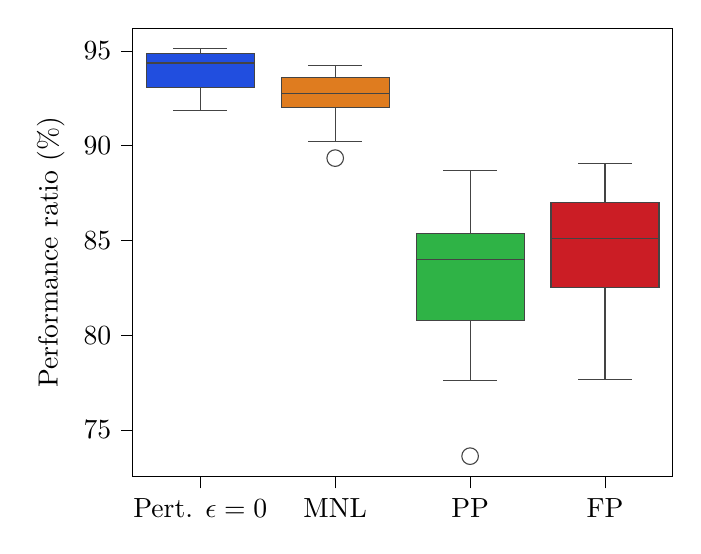
\begin{tikzpicture}

\definecolor{chocolate22312431}{RGB}{223,124,31}
\definecolor{darkgray176}{RGB}{176,176,176}
\definecolor{darkslategray68}{RGB}{68,68,68}
\definecolor{firebrick2032937}{RGB}{203,29,37}
\definecolor{limegreen4717970}{RGB}{47,179,70}
\definecolor{royalblue3378223}{RGB}{33,78,223}

\begin{axis}[
tick align=outside,
tick pos=left,
x grid style={darkgray176},
xmin=-0.5, xmax=3.5,
xtick style={color=black},
xtick={0,1,2,3},
xticklabels={Pert. \(\displaystyle \epsilon=0\),MNL,PP,FP},
y grid style={darkgray176},
ylabel={Performance ratio (\%)},
ymin=72.5467977566071, ymax=96.2003769214691,
ytick style={color=black},
ytick={70,75,80,85,90,95,100},
yticklabels={
  \(\displaystyle {70}\),
  \(\displaystyle {75}\),
  \(\displaystyle {80}\),
  \(\displaystyle {85}\),
  \(\displaystyle {90}\),
  \(\displaystyle {95}\),
  \(\displaystyle {100}\)
}
]
\path [draw=darkslategray68, fill=royalblue3378223]
(axis cs:-0.4,93.0765634615927)
--(axis cs:0.4,93.0765634615927)
--(axis cs:0.4,94.8837217605645)
--(axis cs:-0.4,94.8837217605645)
--(axis cs:-0.4,93.0765634615927)
--cycle;
\addplot [darkslategray68]
table {%
0 93.0765634615927
0 91.8523982442826
};
\addplot [darkslategray68]
table {%
0 94.8837217605645
0 95.1252142321572
};
\addplot [darkslategray68]
table {%
-0.2 91.8523982442826
0.2 91.8523982442826
};
\addplot [darkslategray68]
table {%
-0.2 95.1252142321572
0.2 95.1252142321572
};
\path [draw=darkslategray68, fill=chocolate22312431]
(axis cs:0.6,92.0224894960145)
--(axis cs:1.4,92.0224894960145)
--(axis cs:1.4,93.6162686656397)
--(axis cs:0.6,93.6162686656397)
--(axis cs:0.6,92.0224894960145)
--cycle;
\addplot [darkslategray68]
table {%
1 92.0224894960145
1 90.2346005578498
};
\addplot [darkslategray68]
table {%
1 93.6162686656397
1 94.2259197773107
};
\addplot [darkslategray68]
table {%
0.8 90.2346005578498
1.2 90.2346005578498
};
\addplot [darkslategray68]
table {%
0.8 94.2259197773107
1.2 94.2259197773107
};
\addplot [black, mark=o, mark size=3, mark options={solid,fill opacity=0,draw=darkslategray68}, only marks]
table {%
1 89.347001997502
};
\path [draw=darkslategray68, fill=limegreen4717970]
(axis cs:1.6,80.7656222923379)
--(axis cs:2.4,80.7656222923379)
--(axis cs:2.4,85.3874874430389)
--(axis cs:1.6,85.3874874430389)
--(axis cs:1.6,80.7656222923379)
--cycle;
\addplot [darkslategray68]
table {%
2 80.7656222923379
2 77.6341964522543
};
\addplot [darkslategray68]
table {%
2 85.3874874430389
2 88.7043764630758
};
\addplot [darkslategray68]
table {%
1.8 77.6341964522543
2.2 77.6341964522543
};
\addplot [darkslategray68]
table {%
1.8 88.7043764630758
2.2 88.7043764630758
};
\addplot [black, mark=o, mark size=3, mark options={solid,fill opacity=0,draw=darkslategray68}, only marks]
table {%
2 73.621960445919
};
\path [draw=darkslategray68, fill=firebrick2032937]
(axis cs:2.6,82.5021621714283)
--(axis cs:3.4,82.5021621714283)
--(axis cs:3.4,87.0227157031759)
--(axis cs:2.6,87.0227157031759)
--(axis cs:2.6,82.5021621714283)
--cycle;
\addplot [darkslategray68]
table {%
3 82.5021621714283
3 77.6603881814643
};
\addplot [darkslategray68]
table {%
3 87.0227157031759
3 89.0406873356241
};
\addplot [darkslategray68]
table {%
2.8 77.6603881814643
3.2 77.6603881814643
};
\addplot [darkslategray68]
table {%
2.8 89.0406873356241
3.2 89.0406873356241
};
\addplot [darkslategray68]
table {%
-0.4 94.3656415323535
0.4 94.3656415323535
};
\addplot [darkslategray68]
table {%
0.6 92.7418460931945
1.4 92.7418460931945
};
\addplot [darkslategray68]
table {%
1.6 84.0058825970647
2.4 84.0058825970647
};
\addplot [darkslategray68]
table {%
2.6 85.0975996089361
3.4 85.0975996089361
};
\draw (axis cs:0,66.6334029653916) node[
  scale=0.75,
  anchor=base,
  text=black,
  rotate=0.0
]{\bfseries 94.00};
\draw (axis cs:1,66.6334029653916) node[
  scale=0.75,
  anchor=base,
  text=black,
  rotate=0.0
]{\bfseries 92.61};
\draw (axis cs:2,66.6334029653916) node[
  scale=0.75,
  anchor=base,
  text=black,
  rotate=0.0
]{\bfseries 83.05};
\draw (axis cs:3,66.6334029653916) node[
  scale=0.75,
  anchor=base,
  text=black,
  rotate=0.0
]{\bfseries 84.65};
\draw (axis cs:-1,66.8699387570403) node[
  scale=0.75,
  text=black,
  rotate=0.0
]{\bfseries \textbf{Average:}};
\end{axis}

\end{tikzpicture}
} }}%
    \caption{\textnormal{Performance ratios for synthetic scenarios I.1, I.2, and I.3, which correspond to equal, lower, and higher request arrival rates compared to gig worker arrival rates.}}%
    \label{fig:perf_syn}%
\end{figure}

\noindent \textbf{Performance:} The boxplots in Figure \ref{fig:perf_syn} show the performance ratios across all test set realizations for each of the three sub-scenarios. In Scenario I.1, where the arrival rates of requests and gig workers are equal, our algorithm achieves an average performance ratio of 92.9\% (±3.4\%), compared to 95.1\% (±2.8\%) for the Pert. ($\epsilon=0$) benchmark, which has an inherent advantage over all other benchmarks due to prior and accurate knowledge of gig workers' utilities. The rule based benchmarks achieve a performance of 85.5\% (±4.4\%) for \gls{acr:pp}, and 85.1\% (±4.6\%) for \gls{acr:fp}. Accordingly, our algorithm yields approximately an average improvement of 7.5\% over both benchmarks, while at the same time showing a lower standard deviation. This indicates that our algorithm is particularly effective when the arrival rates are balanced highlighting the stability of our method in this scenario.

In Scenario I.2, where the arrival rate of requests is lower than that of gig workers, our algorithm achieves an average performance ratio of 94.7\% (±2.3\%), compared to 96.1\% (±2.3\%) for the Pert. ($\epsilon=0$), 88.6\% (±3.8\%) for the \gls{acr:pp}, and 88.5\% (±3.7\%) for the \gls{acr:fp} benchmark. Here, the average performance improvement of 6.2\% over \gls{acr:pp} and \gls{acr:fp} highlights our algorithm's capability to maintain a high performance ratio in situations where requests are less frequent. Additionally, our algorithm's standard deviation remains lower than that of both \gls{acr:pp} and \gls{acr:fp}, indicating consistent performance in this scenario as well.

Lastly, in Scenario I.3, where the arrival rate of requests exceeds that of gig workers, our algorithm achieves an average performance ratio of 88.5\% (±1.8\%), compared to 93.2\% (±1.7\%) for the Pert. ($\epsilon=0$), 85.7\% (±3.1\%) for the \gls{acr:pp}, and 86.1\% (±3.7\%) for the \gls{acr:fp} benchmark. In this case, the algorithm only outperforms the \gls{acr:pp} and \gls{acr:fp} benchmarks by an average of 2.5\%. This scenario reveals a lower performance ratio, indicating that while our algorithm remains beneficial, it is less effective in scenarios where the arrival of requests significantly exceeds that of gig workers. We attribute this reduced effectiveness to potential estimation errors in our algorithm, which relies on the \gls{acr:mnl} model for utility predictions. With a high volume of requests, even minor utility estimation errors may amplify across numerous requests, causing greater deviations in performance. This challenge does not affect the Pert. ($\epsilon=0$) benchmark since this benchmark leverages prior knowledge of gig workers’ utilities and remains more robust under these conditions.

Overall, our algorithm consistently outperforms both the \gls{acr:pp} and \gls{acr:fp} benchmarks across all scenarios, yielding improvements between 2.5-7.5\%, with the degree of improvement varying based on the specific arrival rate conditions. We observe a negative gap of 1.4-4.7\% between our algorithm's performance and that of the Pert. ($\epsilon=0$) benchmark. This observed discrepancy can be attributed primarily to errors in estimating the gig worker's utility, and it is particularly pronounced in Scenario I.3, where the lower accuracy of the utility estimator impacts performance more than in the other two scenarios. As expected, the quality of the utility estimator directly influences our algorithm's performance. To further investigate the effect of gig worker utility estimation quality on our algorithm's performance, we conduct a sensitivity analysis over $\epsilon$ in the following.

\noindent \textbf{Result 1:} In a homogeneous gig worker population, our algorithm achieved performance ratios between 88.5\% and 94.7\% across various request arrival rates, consistently outperforming both the \gls{acr:pp} and \gls{acr:fp} benchmarks by 2.5-7.5\%. 

\begin{figure}[t!]%
    \centering
    \fontsize{10}{10}\selectfont
    \includegraphics[width=\textwidth]{figures/synthetic/_perf_ratios_model_comparison_heatmap.pdf}%
    \caption{\textnormal{Performance ratio and \gls{acr:mbe} for \gls{acr:p-pd-vfa} under various perturbation bounds $\epsilon$. The y-axis represents the different perturbation bounds, while the x-axis shows 10 perturbations, each sampled using a unique random seed. The numerical value inside each cell and the size of the circle indicate the achieved performance ratio. Meanwhile, the color gradient of the circles reflects the corresponding MBE of the estimated utilities for each perturbation. The final column shows the average performance ratio and MBE across all random seeds for each perturbation bound.}}
    \label{fig:sens_syn}%
\end{figure}

\noindent \textbf{Sensitivity analysis:} Figure \ref{fig:sens_syn} presents the results from a sensitivity analysis with respect to the estimates of the \gls{acr:mnl} model. Specifically, we evaluate the performance of the \gls{acr:p-pd-vfa} method under varying levels of perturbation. We vary the perturbation bound $\epsilon \in \{2, 4, 6\}$ across 10 different random seeds, each producing a distinct perturbation vector. Our results show that our method remains relatively stable against perturbations that cause underestimation of gig workers' utilities, as characterized by a positive \gls{acr:mbe}. For more details, we refer to Appendix \ref{sec:mbe}. However, when perturbations lead to substantial overestimations, indicated by a strongly negative \gls{acr:mbe}, performance can degrade significantly. In extreme cases almost no requests are accepted, leading to a performance ratio around zero. This aligns with expectations: if the utility model overestimates the utilities, it incorrectly assumes that requests are more attractive to gig workers than they actually are, resulting in insufficient compensation to incentivize acceptance. Conversely, underestimation provides enough compensation to ensure acceptance but reduces revenue, as a lower offer could have sufficed for gig worker incentivization. As expected, increasing the perturbation bound deteriorates performance in all cases, with a more pronounced effect when utilities are overestimated rather than underestimated.

We argue that in practical applications of our algorithm, where \gls{acr:mnl} parameters are estimated using real data, it is more likely for the estimation errors to result in underestimations rather than overestimations. This argument is based on the premise that for a model to systematically overestimate utilities, gig workers must consistently accept requests for compensations lower than their baseline utility for each request. Such occurrences are only observable due to the natural variability in gig workers' utility functions, stemming from the stochastic elements of their decision-making. In contrast, underestimating utility functions is more probable, as this can occur when data is collected under an improper policy, specifically, one that systematically over-offers compensation, prompting gig workers to select the most profitable options. In these scenarios, it becomes challenging to determine the true baseline of gig worker utilities from the data. 

\noindent \textbf{Result 2:} Perturbations to the true \gls{acr:mnl} parameters lead to performance degradation, with more pronounced effects when gig workers' utilities are overestimated.

\subsection{Heterogeneous gig worker population}
\label{sec:res_syn_2}
In the following, we evaluate the impact on algorithmic performance when incorporating knowledge about different gig worker groups compared to cases without such knowledge. To this end, we test two variations of our algorithm. In the first variation, we assume that the platform has no information about the existence of different gig worker groups, thus applying a single \gls{acr:mnl} model across all gig workers. In the second variation, we assume that the platform is aware of different gig worker groups, allowing us to use three separate \gls{acr:mnl} models (Multi \gls{acr:mnl}) to better reflect group-specific preferences. 

\begin{figure}[b!]
    \begin{minipage}{0.62\textwidth}
        \centering
        \subfloat[\centering Single \gls{acr:mnl} model]{{\adjustbox{width=0.49\textwidth}{\includegraphics{figures/momnl/single_MoMNL_diff_all_gig.pdf}} }}%
        \hspace*{0.1cm} 
        \subfloat[\centering Multiple \gls{acr:mnl} models]{{\adjustbox{width=0.49\textwidth}{\includegraphics{figures/momnl/MoMNL_diff_all_gig.pdf}} }}%
        \caption{\textnormal{Difference between true utility and estimated utility when using a single \gls{acr:mnl} model (a) or multiple \gls{acr:mnl} models (b).}}
        \label{fig:mnl_momnl}
    \end{minipage}%
    \hspace*{0.02\textwidth} % Adjust space as needed
    \raisebox{0.1cm}{\begin{minipage}{0.34\textwidth}
        \centering
        \fontsize{10}{10}\selectfont
        \adjustbox{width=0.9\textwidth}{% This file was created with tikzplotlib v0.10.1.
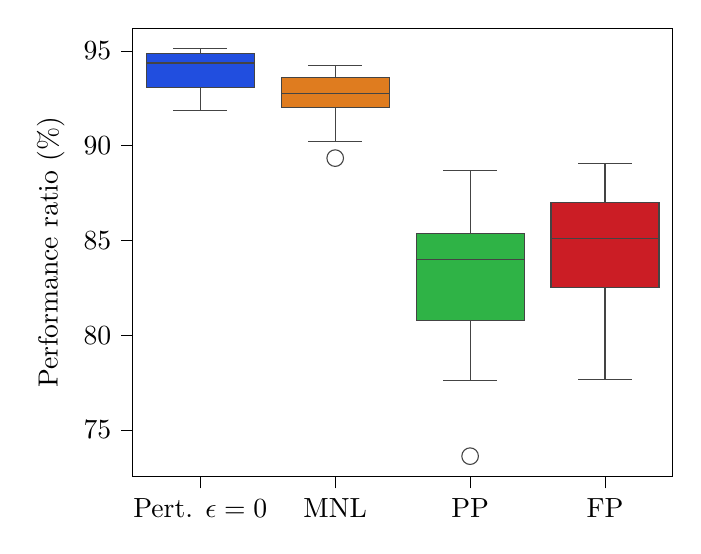
\begin{tikzpicture}

\definecolor{chocolate22312431}{RGB}{223,124,31}
\definecolor{darkgray176}{RGB}{176,176,176}
\definecolor{darkslategray68}{RGB}{68,68,68}
\definecolor{firebrick2032937}{RGB}{203,29,37}
\definecolor{limegreen4717970}{RGB}{47,179,70}
\definecolor{royalblue3378223}{RGB}{33,78,223}

\begin{axis}[
tick align=outside,
tick pos=left,
x grid style={darkgray176},
xmin=-0.5, xmax=3.5,
xtick style={color=black},
xtick={0,1,2,3},
xticklabels={Pert. \(\displaystyle \epsilon=0\),MNL,PP,FP},
y grid style={darkgray176},
ylabel={Performance ratio (\%)},
ymin=72.5467977566071, ymax=96.2003769214691,
ytick style={color=black},
ytick={70,75,80,85,90,95,100},
yticklabels={
  \(\displaystyle {70}\),
  \(\displaystyle {75}\),
  \(\displaystyle {80}\),
  \(\displaystyle {85}\),
  \(\displaystyle {90}\),
  \(\displaystyle {95}\),
  \(\displaystyle {100}\)
}
]
\path [draw=darkslategray68, fill=royalblue3378223]
(axis cs:-0.4,93.0765634615927)
--(axis cs:0.4,93.0765634615927)
--(axis cs:0.4,94.8837217605645)
--(axis cs:-0.4,94.8837217605645)
--(axis cs:-0.4,93.0765634615927)
--cycle;
\addplot [darkslategray68]
table {%
0 93.0765634615927
0 91.8523982442826
};
\addplot [darkslategray68]
table {%
0 94.8837217605645
0 95.1252142321572
};
\addplot [darkslategray68]
table {%
-0.2 91.8523982442826
0.2 91.8523982442826
};
\addplot [darkslategray68]
table {%
-0.2 95.1252142321572
0.2 95.1252142321572
};
\path [draw=darkslategray68, fill=chocolate22312431]
(axis cs:0.6,92.0224894960145)
--(axis cs:1.4,92.0224894960145)
--(axis cs:1.4,93.6162686656397)
--(axis cs:0.6,93.6162686656397)
--(axis cs:0.6,92.0224894960145)
--cycle;
\addplot [darkslategray68]
table {%
1 92.0224894960145
1 90.2346005578498
};
\addplot [darkslategray68]
table {%
1 93.6162686656397
1 94.2259197773107
};
\addplot [darkslategray68]
table {%
0.8 90.2346005578498
1.2 90.2346005578498
};
\addplot [darkslategray68]
table {%
0.8 94.2259197773107
1.2 94.2259197773107
};
\addplot [black, mark=o, mark size=3, mark options={solid,fill opacity=0,draw=darkslategray68}, only marks]
table {%
1 89.347001997502
};
\path [draw=darkslategray68, fill=limegreen4717970]
(axis cs:1.6,80.7656222923379)
--(axis cs:2.4,80.7656222923379)
--(axis cs:2.4,85.3874874430389)
--(axis cs:1.6,85.3874874430389)
--(axis cs:1.6,80.7656222923379)
--cycle;
\addplot [darkslategray68]
table {%
2 80.7656222923379
2 77.6341964522543
};
\addplot [darkslategray68]
table {%
2 85.3874874430389
2 88.7043764630758
};
\addplot [darkslategray68]
table {%
1.8 77.6341964522543
2.2 77.6341964522543
};
\addplot [darkslategray68]
table {%
1.8 88.7043764630758
2.2 88.7043764630758
};
\addplot [black, mark=o, mark size=3, mark options={solid,fill opacity=0,draw=darkslategray68}, only marks]
table {%
2 73.621960445919
};
\path [draw=darkslategray68, fill=firebrick2032937]
(axis cs:2.6,82.5021621714283)
--(axis cs:3.4,82.5021621714283)
--(axis cs:3.4,87.0227157031759)
--(axis cs:2.6,87.0227157031759)
--(axis cs:2.6,82.5021621714283)
--cycle;
\addplot [darkslategray68]
table {%
3 82.5021621714283
3 77.6603881814643
};
\addplot [darkslategray68]
table {%
3 87.0227157031759
3 89.0406873356241
};
\addplot [darkslategray68]
table {%
2.8 77.6603881814643
3.2 77.6603881814643
};
\addplot [darkslategray68]
table {%
2.8 89.0406873356241
3.2 89.0406873356241
};
\addplot [darkslategray68]
table {%
-0.4 94.3656415323535
0.4 94.3656415323535
};
\addplot [darkslategray68]
table {%
0.6 92.7418460931945
1.4 92.7418460931945
};
\addplot [darkslategray68]
table {%
1.6 84.0058825970647
2.4 84.0058825970647
};
\addplot [darkslategray68]
table {%
2.6 85.0975996089361
3.4 85.0975996089361
};
\draw (axis cs:0,66.6334029653916) node[
  scale=0.75,
  anchor=base,
  text=black,
  rotate=0.0
]{\bfseries 94.00};
\draw (axis cs:1,66.6334029653916) node[
  scale=0.75,
  anchor=base,
  text=black,
  rotate=0.0
]{\bfseries 92.61};
\draw (axis cs:2,66.6334029653916) node[
  scale=0.75,
  anchor=base,
  text=black,
  rotate=0.0
]{\bfseries 83.05};
\draw (axis cs:3,66.6334029653916) node[
  scale=0.75,
  anchor=base,
  text=black,
  rotate=0.0
]{\bfseries 84.65};
\draw (axis cs:-1,66.8699387570403) node[
  scale=0.75,
  text=black,
  rotate=0.0
]{\bfseries \textbf{Average:}};
\end{axis}

\end{tikzpicture}
}
        \caption{\textnormal{Performance ratios in Scenario II}}%
        \label{fig:perf_syn_2}%
    \end{minipage}}
\end{figure}

Figure \ref{fig:mnl_momnl} illustrates the difference between the true utility and estimated utility when using either a single \gls{acr:mnl} or three separate \gls{acr:mnl} models. As expected, it is hard to accurately capture the true underlying utility model within a singular \gls{acr:mnl} model (Figure \ref{fig:mnl_momnl}a). The \gls{acr:rmse} between the estimated utility and the true utility is equal to 1.8, 12.7, and 11.7 for each respective group of gig worker, indicating that the predictive accuracy varies significantly among different gig worker groups. When employing a distinct \gls{acr:mnl} model for each group of gig worker, the \gls{acr:rmse} between the estimated utility and the true utility is equal to 2.2, 12.9, and 3.2 for each respective group of gig worker (Figure \ref{fig:mnl_momnl}b). The accuracy of utility estimation for gig worker group 3 has significantly improved, while the performance for gig worker group 1 remains comparable to that of the singular model. However, similar to the singular \gls{acr:mnl} model, the performance for gig worker group 2 remains relatively low, suggesting an inherent difficulty in estimating this group's utility. This difficulty stems from the fact that the groups have varying intrinsic utility levels, and accordingly require varying levels of compensation to be incentivized: specifically, group 2 demonstrates the highest average utility for requests compared to the other two groups (Figure~\ref{fig:utility_scen_2}), indicating that, they require the least compensation on average. As a result, when applying a uniform pricing policy across all gig worker groups during data collection for training the \gls{acr:mnl} model, we tend to overcompensate this group on average to ensure adequate incentives for the other two groups.

\noindent \textbf{Performance:} Figure~\ref{fig:perf_syn_2} shows the distribution of performance ratios across all test set realizations, including benchmarks \gls{acr:pp}, \gls{acr:fp}, and Pert. ($\epsilon=0$), alongside the two variations of our algorithm. When utilizing the correct number of \gls{acr:mnl} models, our algorithm demonstrates an average performance ratio of 89.5\% (±3.1\%), compared to 92.6\% (±3.1\%) for the Pert. ($\epsilon=0$), 79.2\% (±4.3\%) for the \gls{acr:pp}, and 80.4\% (±5.3\%) for the \gls{acr:fp} benchmark. In contrast, when employing a single \gls{acr:mnl} model, the average performance ratio drops significantly to 75.5\% (±9.0\%), and is inferior to all benchmark policies. Our results underscore the importance of having a reliable utility estimator, which requires the platform to understand the characteristics of gig workers to effectively differentiate between various groups. Notably, even though the multi-\gls{acr:mnl} estimator exhibits a relatively high error in estimating the utility for a specific gig worker group, it still manages to achieve satisfactory overall performance. This finding suggests that while having multiple models improves the algorithm's ability to capture utility variations, the platform must also focus on refining the accuracy of the utility estimations across different gig worker groups to further enhance overall performance.

\begin{figure}[t!]%
    \centering
    \fontsize{10}{10}\selectfont
    \includegraphics[width=\textwidth]{figures/momnl/_perf_ratios_model_comparison_heatmap.pdf}%
    \caption{\textnormal{Performance ratio and \gls{acr:mbe} for \gls{acr:p-pd-vfa} under various perturbation bounds $\epsilon$.  We denote the bound as $\epsilon_d$ in the case where only the parameters of gig worker group $d \in \{1,2,3\}$ are perturbed. The y-axis represents the different perturbation bounds, while the x-axis shows 10 perturbations, each sampled using a unique random seed. The numerical value inside each cell and the size of the circle indicate the achieved performance ratio. Meanwhile, the color gradient of the circles reflects the corresponding MBE of the estimated utilities for each perturbation. The final column shows the average performance ratio and MBE across all random seeds for each perturbation bound}}
    \label{fig:sens_syn_2}%
\end{figure}

\noindent \textbf{Result 3:} In a heterogeneous population, our algorithm achieved an average performance ratio of 89.5\%, outperforming both the \gls{acr:pp} and \gls{acr:fp} benchmarks by 9-10\%, when employing the correct number of \gls{acr:mnl} models. Using a single \gls{acr:mnl} model resulted in lower performance (75.5\%), further underscoring the importance of accurate utility estimation when dealing with diverse gig worker groups. 

\noindent \textbf{Sensitivity analysis:} In Figure \ref{fig:sens_syn_2}, we conduct a sensitivity analysis on the \gls{acr:mnl} model estimates by evaluating the performance of \gls{acr:p-pd-vfa} under varying perturbation bounds $\epsilon$. We denote the bound as $\epsilon_d$ in the case where only the parameters of gig worker group $d \in \{1,2,3\}$ are perturbed. Alternatively, we denote the bound as $\epsilon$ when the parameters of all groups are perturbed. As expected, perturbing the parameters of all gig worker groups leads to greater performance degradation, while perturbing the parameters of only one group results in relatively robust, albeit reduced, performance. Although perturbing the utility estimates of individual gig worker groups does negatively impact performance, the degree of degradation is similar across all groups. Consistent with the results from Section \ref{sec:res_syn}, perturbations that lead to overestimation of gig worker utilities have a more severe impact on performance compared to underestimations.

\noindent \textbf{Result 4:} Performance degrades as the accuracy of the gig worker utility estimator worsens, but the extent of degradation is relatively consistent across groups.

\subsection{New York Taxi Data}
\label{sec:res_nyt}
We now apply our algorithm to real-world data from New York taxi services, to test the robustness of the algorithm under more complex, realistic conditions. For gig workers with weak location preferences, the algorithm operates in an environment where gig workers are indifferent with regards to specific locations, thus representing simpler, non-rigid settings. In contrast, strong location preferences introduce additional complexity, as gig workers prioritize particular areas. This analysis provides deeper insights into the algorithm's behavior in cases where gig worker preferences over specific locations play a more decisive role in request acceptance.

\begin{figure}[b!]
    \centering
    \begin{minipage}{0.48\textwidth}
        \centering
        \fontsize{10}{10}\selectfont
        \subfloat[\centering Grouped by pickup location (weak preference)]{{\includegraphics[width=0.48\textwidth]{figures/nyt/NYT_weak_diff_pickup_location.pdf}}}%
        \hspace*{0.1cm}
        \subfloat[\centering Grouped by dropoff location (weak preference)]{{\includegraphics[width=0.48\textwidth]{figures/nyt/NYT_weak_diff_dropoff_location.pdf}}}%
    \end{minipage}\hfill
    \begin{minipage}{0.48\textwidth}
        \centering
        \fontsize{10}{10}\selectfont
        \subfloat[\centering Grouped by pickup location (strong preference)]{{\includegraphics[width=0.48\textwidth]{figures/nyt_strong/NYT_strong_diff_pickup_location.pdf}}}%
        \hspace*{0.1cm}
        \subfloat[\centering Grouped by dropoff location (strong preference)]{{\includegraphics[width=0.48\textwidth]{figures/nyt_strong/NYT_strong_diff_dropoff_location.pdf}}}%
    \end{minipage}
    \caption{\textnormal{Difference between true utility and estimated utility grouped by pickup and dropoff locations for NYT data, with gig workers exhibiting weak location preference in (a) and (b), and strong location preference in (c) and (d).}}
    \label{fig:nyt_combined_mnl}
\end{figure}

The trained MNL model’s utility estimation accuracy varies across preference scenarios. Figure \ref{fig:nyt_combined_mnl} show histograms depicting the difference between the true and the estimated utility for NYT data with weak and strong location preference gig workers. In the weak preferences scenario (see Figure \ref{fig:nyt_combined_mnl}a\&b), the \gls{acr:mnl} model achieves a \gls{acr:rmse} of 1.8 and shows a slight average underestimation of request utilities with an overall \gls{acr:mbe} of 1.6. We do not observe any distinct pattern where requests with specific pickup or dropoff locations are significantly over- or under-estimated. In the strong preference scenario (Figure \ref{fig:nyt_combined_mnl}c\&d), the model faces greater complexity in estimating the \gls{acr:mnl} parameters. Despite the \gls{acr:mnl} model achieving a reasonably good \gls{acr:rmse} of 2.5 and an overall \gls{acr:mbe} of 0.08, we observe varying biases in the utility estimation of different subgroups of requests. For instance, we observe an overestimation of utilities for requests with dropoff location 1, whereas we observe an underestimation for other dropoff locations (Figure \ref{fig:nyt_combined_mnl}d). This scenario is one of the most challenging cases for accurate utility estimation, as it has the most divergent distribution in terms of utilities.

\begin{figure}[t!]
    \centering
    \captionsetup[subfloat]{labelformat=empty}
    \fontsize{9}{9}\selectfont
    % Left side: Single subfigure
    \begin{minipage}{0.32\textwidth}
        \centering
        \subfloat[\vspace{-0.05cm}]{\adjustbox{width=\textwidth}{ % This file was created with tikzplotlib v0.10.1.
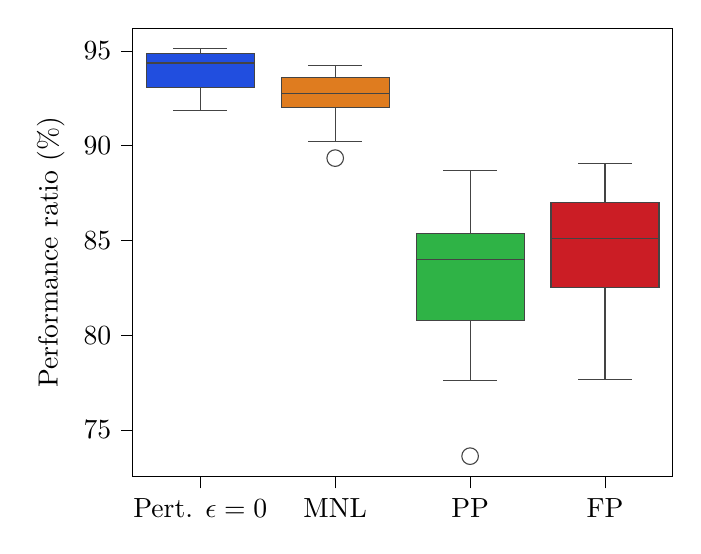
\begin{tikzpicture}

\definecolor{chocolate22312431}{RGB}{223,124,31}
\definecolor{darkgray176}{RGB}{176,176,176}
\definecolor{darkslategray68}{RGB}{68,68,68}
\definecolor{firebrick2032937}{RGB}{203,29,37}
\definecolor{limegreen4717970}{RGB}{47,179,70}
\definecolor{royalblue3378223}{RGB}{33,78,223}

\begin{axis}[
tick align=outside,
tick pos=left,
x grid style={darkgray176},
xmin=-0.5, xmax=3.5,
xtick style={color=black},
xtick={0,1,2,3},
xticklabels={Pert. \(\displaystyle \epsilon=0\),MNL,PP,FP},
y grid style={darkgray176},
ylabel={Performance ratio (\%)},
ymin=72.5467977566071, ymax=96.2003769214691,
ytick style={color=black},
ytick={70,75,80,85,90,95,100},
yticklabels={
  \(\displaystyle {70}\),
  \(\displaystyle {75}\),
  \(\displaystyle {80}\),
  \(\displaystyle {85}\),
  \(\displaystyle {90}\),
  \(\displaystyle {95}\),
  \(\displaystyle {100}\)
}
]
\path [draw=darkslategray68, fill=royalblue3378223]
(axis cs:-0.4,93.0765634615927)
--(axis cs:0.4,93.0765634615927)
--(axis cs:0.4,94.8837217605645)
--(axis cs:-0.4,94.8837217605645)
--(axis cs:-0.4,93.0765634615927)
--cycle;
\addplot [darkslategray68]
table {%
0 93.0765634615927
0 91.8523982442826
};
\addplot [darkslategray68]
table {%
0 94.8837217605645
0 95.1252142321572
};
\addplot [darkslategray68]
table {%
-0.2 91.8523982442826
0.2 91.8523982442826
};
\addplot [darkslategray68]
table {%
-0.2 95.1252142321572
0.2 95.1252142321572
};
\path [draw=darkslategray68, fill=chocolate22312431]
(axis cs:0.6,92.0224894960145)
--(axis cs:1.4,92.0224894960145)
--(axis cs:1.4,93.6162686656397)
--(axis cs:0.6,93.6162686656397)
--(axis cs:0.6,92.0224894960145)
--cycle;
\addplot [darkslategray68]
table {%
1 92.0224894960145
1 90.2346005578498
};
\addplot [darkslategray68]
table {%
1 93.6162686656397
1 94.2259197773107
};
\addplot [darkslategray68]
table {%
0.8 90.2346005578498
1.2 90.2346005578498
};
\addplot [darkslategray68]
table {%
0.8 94.2259197773107
1.2 94.2259197773107
};
\addplot [black, mark=o, mark size=3, mark options={solid,fill opacity=0,draw=darkslategray68}, only marks]
table {%
1 89.347001997502
};
\path [draw=darkslategray68, fill=limegreen4717970]
(axis cs:1.6,80.7656222923379)
--(axis cs:2.4,80.7656222923379)
--(axis cs:2.4,85.3874874430389)
--(axis cs:1.6,85.3874874430389)
--(axis cs:1.6,80.7656222923379)
--cycle;
\addplot [darkslategray68]
table {%
2 80.7656222923379
2 77.6341964522543
};
\addplot [darkslategray68]
table {%
2 85.3874874430389
2 88.7043764630758
};
\addplot [darkslategray68]
table {%
1.8 77.6341964522543
2.2 77.6341964522543
};
\addplot [darkslategray68]
table {%
1.8 88.7043764630758
2.2 88.7043764630758
};
\addplot [black, mark=o, mark size=3, mark options={solid,fill opacity=0,draw=darkslategray68}, only marks]
table {%
2 73.621960445919
};
\path [draw=darkslategray68, fill=firebrick2032937]
(axis cs:2.6,82.5021621714283)
--(axis cs:3.4,82.5021621714283)
--(axis cs:3.4,87.0227157031759)
--(axis cs:2.6,87.0227157031759)
--(axis cs:2.6,82.5021621714283)
--cycle;
\addplot [darkslategray68]
table {%
3 82.5021621714283
3 77.6603881814643
};
\addplot [darkslategray68]
table {%
3 87.0227157031759
3 89.0406873356241
};
\addplot [darkslategray68]
table {%
2.8 77.6603881814643
3.2 77.6603881814643
};
\addplot [darkslategray68]
table {%
2.8 89.0406873356241
3.2 89.0406873356241
};
\addplot [darkslategray68]
table {%
-0.4 94.3656415323535
0.4 94.3656415323535
};
\addplot [darkslategray68]
table {%
0.6 92.7418460931945
1.4 92.7418460931945
};
\addplot [darkslategray68]
table {%
1.6 84.0058825970647
2.4 84.0058825970647
};
\addplot [darkslategray68]
table {%
2.6 85.0975996089361
3.4 85.0975996089361
};
\draw (axis cs:0,66.6334029653916) node[
  scale=0.75,
  anchor=base,
  text=black,
  rotate=0.0
]{\bfseries 94.00};
\draw (axis cs:1,66.6334029653916) node[
  scale=0.75,
  anchor=base,
  text=black,
  rotate=0.0
]{\bfseries 92.61};
\draw (axis cs:2,66.6334029653916) node[
  scale=0.75,
  anchor=base,
  text=black,
  rotate=0.0
]{\bfseries 83.05};
\draw (axis cs:3,66.6334029653916) node[
  scale=0.75,
  anchor=base,
  text=black,
  rotate=0.0
]{\bfseries 84.65};
\draw (axis cs:-1,66.8699387570403) node[
  scale=0.75,
  text=black,
  rotate=0.0
]{\bfseries \textbf{Average:}};
\end{axis}

\end{tikzpicture}
}}
        \caption{\textnormal{Performance ratios for NYT data (weak preference)}}
        \label{fig:perf_nyt_weak}
    \end{minipage}
    \captionsetup[subfloat]{labelformat=parens} % Reset back to default
    \hspace*{0.1cm}
    % Right side: Two subfigures side by side
    \begin{minipage}{0.64\textwidth}
        \centering
        \subfloat[\centering Difference in offered compensation]{{\adjustbox{width=0.49\textwidth}{% This file was created with tikzplotlib v0.10.1.
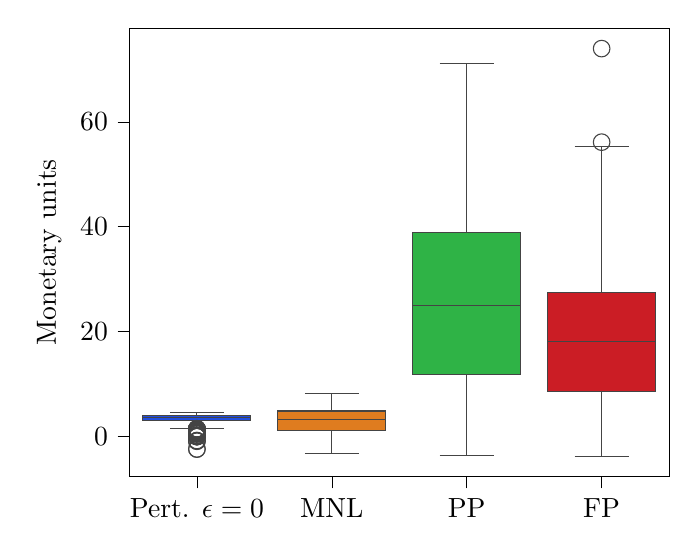
\begin{tikzpicture}

\definecolor{chocolate22312431}{RGB}{223,124,31}
\definecolor{darkgray176}{RGB}{176,176,176}
\definecolor{darkslategray68}{RGB}{68,68,68}
\definecolor{firebrick2032937}{RGB}{203,29,37}
\definecolor{limegreen4717970}{RGB}{47,179,70}
\definecolor{royalblue3378223}{RGB}{33,78,223}

\begin{axis}[
tick align=outside,
tick pos=left,
x grid style={darkgray176},
xmin=-0.5, xmax=3.5,
xtick style={color=black},
xtick={0,1,2,3},
xticklabels={Pert. \(\displaystyle \epsilon=0\),MNL,PP,FP},
y grid style={darkgray176},
ylabel={Monetary units},
ymin=-7.72179203033447, ymax=77.8589876174927,
ytick style={color=black},
ytick={-20,0,20,40,60,80},
yticklabels={
  \(\displaystyle {\ensuremath{-}20}\),
  \(\displaystyle {0}\),
  \(\displaystyle {20}\),
  \(\displaystyle {40}\),
  \(\displaystyle {60}\),
  \(\displaystyle {80}\)
}
]
\path [draw=darkslategray68, fill=royalblue3378223]
(axis cs:-0.4,2.9080810546875)
--(axis cs:0.4,2.9080810546875)
--(axis cs:0.4,3.87141418457031)
--(axis cs:-0.4,3.87141418457031)
--(axis cs:-0.4,2.9080810546875)
--cycle;
\addplot [darkslategray68]
table {%
0 2.9080810546875
0 1.46649169921875
};
\addplot [darkslategray68]
table {%
0 3.87141418457031
0 4.56305313110352
};
\addplot [darkslategray68]
table {%
-0.2 1.46649169921875
0.2 1.46649169921875
};
\addplot [darkslategray68]
table {%
-0.2 4.56305313110352
0.2 4.56305313110352
};
\addplot [black, mark=o, mark size=3, mark options={solid,fill opacity=0,draw=darkslategray68}, only marks]
table {%
0 1.31788635253906
0 1.15647888183594
0 -0.979782104492188
0 0.157768249511719
0 0.0550308227539062
0 0.712020874023438
0 0.814285278320312
0 0.712867736816406
0 0.907318115234375
0 1.04023742675781
0 0.919090270996094
0 1.3988037109375
0 1.16722869873047
0 1.21726989746094
0 0.101913452148438
0 0.631832122802734
0 1.10314178466797
0 1.32956695556641
0 0.535453796386719
0 1.34599304199219
0 0.836349487304688
0 1.05873107910156
0 0.913238525390625
0 -0.0850448608398438
0 -0.017578125
0 -0.0562362670898438
0 1.41719055175781
0 0.717041015625
0 1.29923248291016
0 1.07136917114258
0 -2.47638702392578
0 -0.09478759765625
0 0.164253234863281
0 -0.094573974609375
0 0.803794860839844
0 -0.842056274414062
0 -2.45515441894531
0 0.494766235351562
0 -0.927444458007812
0 0.393043518066406
0 0.828407287597656
0 1.25785827636719
0 1.23259735107422
0 1.05279541015625
0 0.796051025390625
0 1.30381774902344
0 0.734695434570312
0 1.30718231201172
};
\path [draw=darkslategray68, fill=chocolate22312431]
(axis cs:0.6,1.12636947631836)
--(axis cs:1.4,1.12636947631836)
--(axis cs:1.4,4.80079746246338)
--(axis cs:0.6,4.80079746246338)
--(axis cs:0.6,1.12636947631836)
--cycle;
\addplot [darkslategray68]
table {%
1 1.12636947631836
1 -3.25681304931641
};
\addplot [darkslategray68]
table {%
1 4.80079746246338
1 8.09512710571289
};
\addplot [darkslategray68]
table {%
0.8 -3.25681304931641
1.2 -3.25681304931641
};
\addplot [darkslategray68]
table {%
0.8 8.09512710571289
1.2 8.09512710571289
};
\path [draw=darkslategray68, fill=limegreen4717970]
(axis cs:1.6,11.7126359939575)
--(axis cs:2.4,11.7126359939575)
--(axis cs:2.4,38.8348731994629)
--(axis cs:1.6,38.8348731994629)
--(axis cs:1.6,11.7126359939575)
--cycle;
\addplot [darkslategray68]
table {%
2 11.7126359939575
2 -3.72576141357422
};
\addplot [darkslategray68]
table {%
2 38.8348731994629
2 71.0504455566406
};
\addplot [darkslategray68]
table {%
1.8 -3.72576141357422
2.2 -3.72576141357422
};
\addplot [darkslategray68]
table {%
1.8 71.0504455566406
2.2 71.0504455566406
};
\path [draw=darkslategray68, fill=firebrick2032937]
(axis cs:2.6,8.43429946899414)
--(axis cs:3.4,8.43429946899414)
--(axis cs:3.4,27.4146118164062)
--(axis cs:2.6,27.4146118164062)
--(axis cs:2.6,8.43429946899414)
--cycle;
\addplot [darkslategray68]
table {%
3 8.43429946899414
3 -3.83175659179688
};
\addplot [darkslategray68]
table {%
3 27.4146118164062
3 55.3362007141113
};
\addplot [darkslategray68]
table {%
2.8 -3.83175659179688
3.2 -3.83175659179688
};
\addplot [darkslategray68]
table {%
2.8 55.3362007141113
3.2 55.3362007141113
};
\addplot [black, mark=o, mark size=3, mark options={solid,fill opacity=0,draw=darkslategray68}, only marks]
table {%
3 73.9689521789551
3 56.1101303100586
};
\addplot [darkslategray68]
table {%
-0.4 3.49254608154297
0.4 3.49254608154297
};
\addplot [darkslategray68]
table {%
0.6 3.0895824432373
1.4 3.0895824432373
};
\addplot [darkslategray68]
table {%
1.6 24.8769016265869
2.4 24.8769016265869
};
\addplot [darkslategray68]
table {%
2.6 18.0128326416016
3.4 18.0128326416016
};
\end{axis}

\end{tikzpicture}
}}}%
        \hspace*{0.1cm} 
        \subfloat[\centering Percentage of utilized gig workers]{{\adjustbox{width=0.49\textwidth}{% This file was created with tikzplotlib v0.10.1.
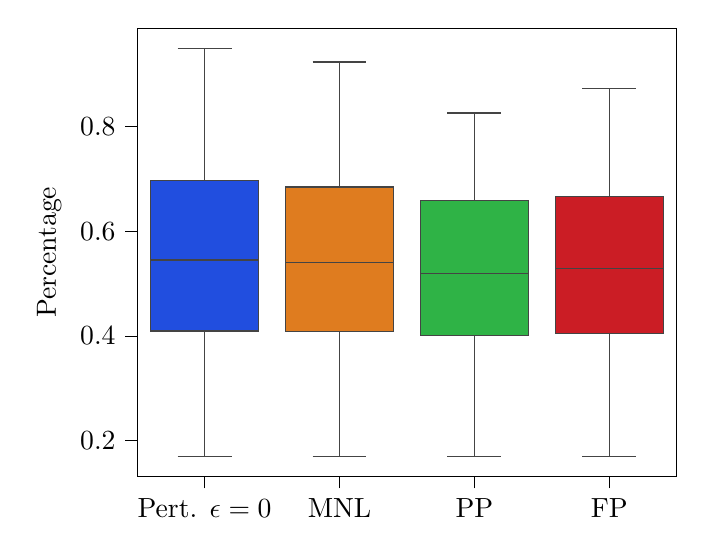
\begin{tikzpicture}

\definecolor{chocolate22312431}{RGB}{223,124,31}
\definecolor{darkgray176}{RGB}{176,176,176}
\definecolor{darkslategray68}{RGB}{68,68,68}
\definecolor{firebrick2032937}{RGB}{203,29,37}
\definecolor{limegreen4717970}{RGB}{47,179,70}
\definecolor{royalblue3378223}{RGB}{33,78,223}

\begin{axis}[
tick align=outside,
tick pos=left,
x grid style={darkgray176},
xmin=-0.5, xmax=3.5,
xtick style={color=black},
xtick={0,1,2,3},
xticklabels={Pert. \(\displaystyle \epsilon=0\),MNL,PP,FP},
y grid style={darkgray176},
ylabel={Percentage},
ymin=0.131064102564103, ymax=0.987653846153846,
ytick style={color=black},
ytick={0,0.2,0.4,0.6,0.8,1},
yticklabels={
  \(\displaystyle {0.0}\),
  \(\displaystyle {0.2}\),
  \(\displaystyle {0.4}\),
  \(\displaystyle {0.6}\),
  \(\displaystyle {0.8}\),
  \(\displaystyle {1.0}\)
}
]
\path [draw=darkslategray68, fill=royalblue3378223]
(axis cs:-0.4,0.409082500924898)
--(axis cs:0.4,0.409082500924898)
--(axis cs:0.4,0.697389063200359)
--(axis cs:-0.4,0.697389063200359)
--(axis cs:-0.4,0.409082500924898)
--cycle;
\addplot [darkslategray68]
table {%
0 0.409082500924898
0 0.17
};
\addplot [darkslategray68]
table {%
0 0.697389063200359
0 0.948717948717949
};
\addplot [darkslategray68]
table {%
-0.2 0.17
0.2 0.17
};
\addplot [darkslategray68]
table {%
-0.2 0.948717948717949
0.2 0.948717948717949
};
\path [draw=darkslategray68, fill=chocolate22312431]
(axis cs:0.6,0.407476686185209)
--(axis cs:1.4,0.407476686185209)
--(axis cs:1.4,0.684222321828776)
--(axis cs:0.6,0.684222321828776)
--(axis cs:0.6,0.407476686185209)
--cycle;
\addplot [darkslategray68]
table {%
1 0.407476686185209
1 0.17
};
\addplot [darkslategray68]
table {%
1 0.684222321828776
1 0.923076923076923
};
\addplot [darkslategray68]
table {%
0.8 0.17
1.2 0.17
};
\addplot [darkslategray68]
table {%
0.8 0.923076923076923
1.2 0.923076923076923
};
\path [draw=darkslategray68, fill=limegreen4717970]
(axis cs:1.6,0.400401214487096)
--(axis cs:2.4,0.400401214487096)
--(axis cs:2.4,0.659233527566114)
--(axis cs:1.6,0.659233527566114)
--(axis cs:1.6,0.400401214487096)
--cycle;
\addplot [darkslategray68]
table {%
2 0.400401214487096
2 0.17
};
\addplot [darkslategray68]
table {%
2 0.659233527566114
2 0.825581395348837
};
\addplot [darkslategray68]
table {%
1.8 0.17
2.2 0.17
};
\addplot [darkslategray68]
table {%
1.8 0.825581395348837
2.2 0.825581395348837
};
\path [draw=darkslategray68, fill=firebrick2032937]
(axis cs:2.6,0.404603122966818)
--(axis cs:3.4,0.404603122966818)
--(axis cs:3.4,0.665313299232737)
--(axis cs:2.6,0.665313299232737)
--(axis cs:2.6,0.404603122966818)
--cycle;
\addplot [darkslategray68]
table {%
3 0.404603122966818
3 0.17
};
\addplot [darkslategray68]
table {%
3 0.665313299232737
3 0.872093023255814
};
\addplot [darkslategray68]
table {%
2.8 0.17
3.2 0.17
};
\addplot [darkslategray68]
table {%
2.8 0.872093023255814
3.2 0.872093023255814
};
\addplot [darkslategray68]
table {%
-0.4 0.544820336391437
0.4 0.544820336391437
};
\addplot [darkslategray68]
table {%
0.6 0.539299242424242
1.4 0.539299242424242
};
\addplot [darkslategray68]
table {%
1.6 0.519677033492823
2.4 0.519677033492823
};
\addplot [darkslategray68]
table {%
2.6 0.527935606060606
3.4 0.527935606060606
};
\end{axis}

\end{tikzpicture}
}}}%
        \caption{\textnormal{Difference in offered compensation from true utility (a) and percentage of utilized gig workers (b) for NYT data (weak preference).}}
        \label{fig:comp_nyt_weak}
    \end{minipage}
\end{figure}
\begin{figure}[t!]
    \centering
    \captionsetup[subfloat]{labelformat=empty}
    \fontsize{9}{9}\selectfont
    % Left side: Single subfigure
    \begin{minipage}{0.32\textwidth}
        \centering
        \subfloat[\vspace{-0.05cm}]{\adjustbox{width=\textwidth}{% This file was created with tikzplotlib v0.10.1.
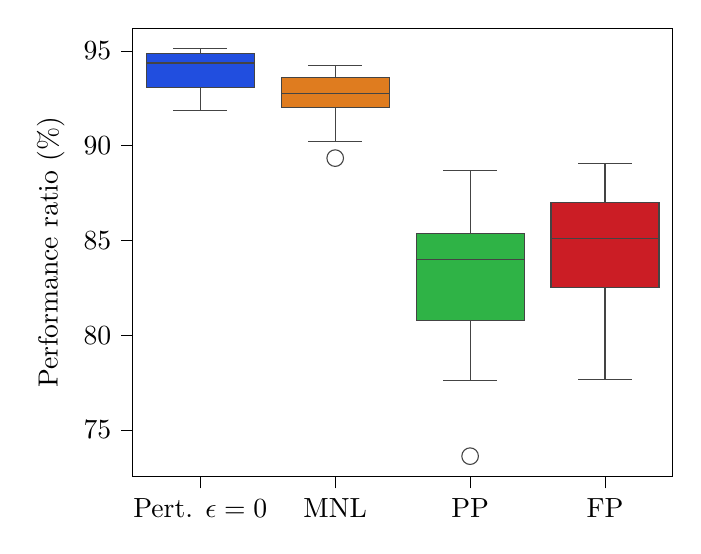
\begin{tikzpicture}

\definecolor{chocolate22312431}{RGB}{223,124,31}
\definecolor{darkgray176}{RGB}{176,176,176}
\definecolor{darkslategray68}{RGB}{68,68,68}
\definecolor{firebrick2032937}{RGB}{203,29,37}
\definecolor{limegreen4717970}{RGB}{47,179,70}
\definecolor{royalblue3378223}{RGB}{33,78,223}

\begin{axis}[
tick align=outside,
tick pos=left,
x grid style={darkgray176},
xmin=-0.5, xmax=3.5,
xtick style={color=black},
xtick={0,1,2,3},
xticklabels={Pert. \(\displaystyle \epsilon=0\),MNL,PP,FP},
y grid style={darkgray176},
ylabel={Performance ratio (\%)},
ymin=72.5467977566071, ymax=96.2003769214691,
ytick style={color=black},
ytick={70,75,80,85,90,95,100},
yticklabels={
  \(\displaystyle {70}\),
  \(\displaystyle {75}\),
  \(\displaystyle {80}\),
  \(\displaystyle {85}\),
  \(\displaystyle {90}\),
  \(\displaystyle {95}\),
  \(\displaystyle {100}\)
}
]
\path [draw=darkslategray68, fill=royalblue3378223]
(axis cs:-0.4,93.0765634615927)
--(axis cs:0.4,93.0765634615927)
--(axis cs:0.4,94.8837217605645)
--(axis cs:-0.4,94.8837217605645)
--(axis cs:-0.4,93.0765634615927)
--cycle;
\addplot [darkslategray68]
table {%
0 93.0765634615927
0 91.8523982442826
};
\addplot [darkslategray68]
table {%
0 94.8837217605645
0 95.1252142321572
};
\addplot [darkslategray68]
table {%
-0.2 91.8523982442826
0.2 91.8523982442826
};
\addplot [darkslategray68]
table {%
-0.2 95.1252142321572
0.2 95.1252142321572
};
\path [draw=darkslategray68, fill=chocolate22312431]
(axis cs:0.6,92.0224894960145)
--(axis cs:1.4,92.0224894960145)
--(axis cs:1.4,93.6162686656397)
--(axis cs:0.6,93.6162686656397)
--(axis cs:0.6,92.0224894960145)
--cycle;
\addplot [darkslategray68]
table {%
1 92.0224894960145
1 90.2346005578498
};
\addplot [darkslategray68]
table {%
1 93.6162686656397
1 94.2259197773107
};
\addplot [darkslategray68]
table {%
0.8 90.2346005578498
1.2 90.2346005578498
};
\addplot [darkslategray68]
table {%
0.8 94.2259197773107
1.2 94.2259197773107
};
\addplot [black, mark=o, mark size=3, mark options={solid,fill opacity=0,draw=darkslategray68}, only marks]
table {%
1 89.347001997502
};
\path [draw=darkslategray68, fill=limegreen4717970]
(axis cs:1.6,80.7656222923379)
--(axis cs:2.4,80.7656222923379)
--(axis cs:2.4,85.3874874430389)
--(axis cs:1.6,85.3874874430389)
--(axis cs:1.6,80.7656222923379)
--cycle;
\addplot [darkslategray68]
table {%
2 80.7656222923379
2 77.6341964522543
};
\addplot [darkslategray68]
table {%
2 85.3874874430389
2 88.7043764630758
};
\addplot [darkslategray68]
table {%
1.8 77.6341964522543
2.2 77.6341964522543
};
\addplot [darkslategray68]
table {%
1.8 88.7043764630758
2.2 88.7043764630758
};
\addplot [black, mark=o, mark size=3, mark options={solid,fill opacity=0,draw=darkslategray68}, only marks]
table {%
2 73.621960445919
};
\path [draw=darkslategray68, fill=firebrick2032937]
(axis cs:2.6,82.5021621714283)
--(axis cs:3.4,82.5021621714283)
--(axis cs:3.4,87.0227157031759)
--(axis cs:2.6,87.0227157031759)
--(axis cs:2.6,82.5021621714283)
--cycle;
\addplot [darkslategray68]
table {%
3 82.5021621714283
3 77.6603881814643
};
\addplot [darkslategray68]
table {%
3 87.0227157031759
3 89.0406873356241
};
\addplot [darkslategray68]
table {%
2.8 77.6603881814643
3.2 77.6603881814643
};
\addplot [darkslategray68]
table {%
2.8 89.0406873356241
3.2 89.0406873356241
};
\addplot [darkslategray68]
table {%
-0.4 94.3656415323535
0.4 94.3656415323535
};
\addplot [darkslategray68]
table {%
0.6 92.7418460931945
1.4 92.7418460931945
};
\addplot [darkslategray68]
table {%
1.6 84.0058825970647
2.4 84.0058825970647
};
\addplot [darkslategray68]
table {%
2.6 85.0975996089361
3.4 85.0975996089361
};
\draw (axis cs:0,66.6334029653916) node[
  scale=0.75,
  anchor=base,
  text=black,
  rotate=0.0
]{\bfseries 94.00};
\draw (axis cs:1,66.6334029653916) node[
  scale=0.75,
  anchor=base,
  text=black,
  rotate=0.0
]{\bfseries 92.61};
\draw (axis cs:2,66.6334029653916) node[
  scale=0.75,
  anchor=base,
  text=black,
  rotate=0.0
]{\bfseries 83.05};
\draw (axis cs:3,66.6334029653916) node[
  scale=0.75,
  anchor=base,
  text=black,
  rotate=0.0
]{\bfseries 84.65};
\draw (axis cs:-1,66.8699387570403) node[
  scale=0.75,
  text=black,
  rotate=0.0
]{\bfseries \textbf{Average:}};
\end{axis}

\end{tikzpicture}
}}
        \caption{\textnormal{Performance ratios for NYT data (strong preference)}}
        \label{fig:perf_nyt_strong}
    \end{minipage}%
    \captionsetup[subfloat]{labelformat=parens} % Reset back to default
    \hspace*{0.1cm}
    % Right side: Two subfigures side by side
    \begin{minipage}{0.64\textwidth}
        \centering
        \subfloat[\centering Difference in offered compensation]{{\adjustbox{width=0.49\textwidth}{% This file was created with tikzplotlib v0.10.1.
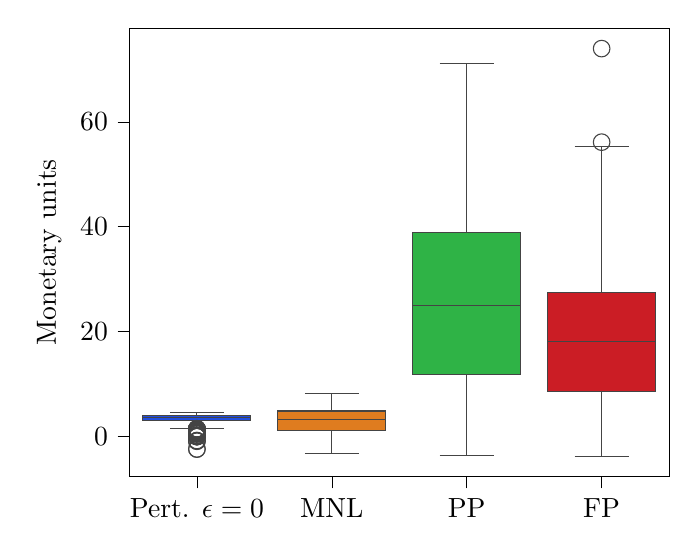
\begin{tikzpicture}

\definecolor{chocolate22312431}{RGB}{223,124,31}
\definecolor{darkgray176}{RGB}{176,176,176}
\definecolor{darkslategray68}{RGB}{68,68,68}
\definecolor{firebrick2032937}{RGB}{203,29,37}
\definecolor{limegreen4717970}{RGB}{47,179,70}
\definecolor{royalblue3378223}{RGB}{33,78,223}

\begin{axis}[
tick align=outside,
tick pos=left,
x grid style={darkgray176},
xmin=-0.5, xmax=3.5,
xtick style={color=black},
xtick={0,1,2,3},
xticklabels={Pert. \(\displaystyle \epsilon=0\),MNL,PP,FP},
y grid style={darkgray176},
ylabel={Monetary units},
ymin=-7.72179203033447, ymax=77.8589876174927,
ytick style={color=black},
ytick={-20,0,20,40,60,80},
yticklabels={
  \(\displaystyle {\ensuremath{-}20}\),
  \(\displaystyle {0}\),
  \(\displaystyle {20}\),
  \(\displaystyle {40}\),
  \(\displaystyle {60}\),
  \(\displaystyle {80}\)
}
]
\path [draw=darkslategray68, fill=royalblue3378223]
(axis cs:-0.4,2.9080810546875)
--(axis cs:0.4,2.9080810546875)
--(axis cs:0.4,3.87141418457031)
--(axis cs:-0.4,3.87141418457031)
--(axis cs:-0.4,2.9080810546875)
--cycle;
\addplot [darkslategray68]
table {%
0 2.9080810546875
0 1.46649169921875
};
\addplot [darkslategray68]
table {%
0 3.87141418457031
0 4.56305313110352
};
\addplot [darkslategray68]
table {%
-0.2 1.46649169921875
0.2 1.46649169921875
};
\addplot [darkslategray68]
table {%
-0.2 4.56305313110352
0.2 4.56305313110352
};
\addplot [black, mark=o, mark size=3, mark options={solid,fill opacity=0,draw=darkslategray68}, only marks]
table {%
0 1.31788635253906
0 1.15647888183594
0 -0.979782104492188
0 0.157768249511719
0 0.0550308227539062
0 0.712020874023438
0 0.814285278320312
0 0.712867736816406
0 0.907318115234375
0 1.04023742675781
0 0.919090270996094
0 1.3988037109375
0 1.16722869873047
0 1.21726989746094
0 0.101913452148438
0 0.631832122802734
0 1.10314178466797
0 1.32956695556641
0 0.535453796386719
0 1.34599304199219
0 0.836349487304688
0 1.05873107910156
0 0.913238525390625
0 -0.0850448608398438
0 -0.017578125
0 -0.0562362670898438
0 1.41719055175781
0 0.717041015625
0 1.29923248291016
0 1.07136917114258
0 -2.47638702392578
0 -0.09478759765625
0 0.164253234863281
0 -0.094573974609375
0 0.803794860839844
0 -0.842056274414062
0 -2.45515441894531
0 0.494766235351562
0 -0.927444458007812
0 0.393043518066406
0 0.828407287597656
0 1.25785827636719
0 1.23259735107422
0 1.05279541015625
0 0.796051025390625
0 1.30381774902344
0 0.734695434570312
0 1.30718231201172
};
\path [draw=darkslategray68, fill=chocolate22312431]
(axis cs:0.6,1.12636947631836)
--(axis cs:1.4,1.12636947631836)
--(axis cs:1.4,4.80079746246338)
--(axis cs:0.6,4.80079746246338)
--(axis cs:0.6,1.12636947631836)
--cycle;
\addplot [darkslategray68]
table {%
1 1.12636947631836
1 -3.25681304931641
};
\addplot [darkslategray68]
table {%
1 4.80079746246338
1 8.09512710571289
};
\addplot [darkslategray68]
table {%
0.8 -3.25681304931641
1.2 -3.25681304931641
};
\addplot [darkslategray68]
table {%
0.8 8.09512710571289
1.2 8.09512710571289
};
\path [draw=darkslategray68, fill=limegreen4717970]
(axis cs:1.6,11.7126359939575)
--(axis cs:2.4,11.7126359939575)
--(axis cs:2.4,38.8348731994629)
--(axis cs:1.6,38.8348731994629)
--(axis cs:1.6,11.7126359939575)
--cycle;
\addplot [darkslategray68]
table {%
2 11.7126359939575
2 -3.72576141357422
};
\addplot [darkslategray68]
table {%
2 38.8348731994629
2 71.0504455566406
};
\addplot [darkslategray68]
table {%
1.8 -3.72576141357422
2.2 -3.72576141357422
};
\addplot [darkslategray68]
table {%
1.8 71.0504455566406
2.2 71.0504455566406
};
\path [draw=darkslategray68, fill=firebrick2032937]
(axis cs:2.6,8.43429946899414)
--(axis cs:3.4,8.43429946899414)
--(axis cs:3.4,27.4146118164062)
--(axis cs:2.6,27.4146118164062)
--(axis cs:2.6,8.43429946899414)
--cycle;
\addplot [darkslategray68]
table {%
3 8.43429946899414
3 -3.83175659179688
};
\addplot [darkslategray68]
table {%
3 27.4146118164062
3 55.3362007141113
};
\addplot [darkslategray68]
table {%
2.8 -3.83175659179688
3.2 -3.83175659179688
};
\addplot [darkslategray68]
table {%
2.8 55.3362007141113
3.2 55.3362007141113
};
\addplot [black, mark=o, mark size=3, mark options={solid,fill opacity=0,draw=darkslategray68}, only marks]
table {%
3 73.9689521789551
3 56.1101303100586
};
\addplot [darkslategray68]
table {%
-0.4 3.49254608154297
0.4 3.49254608154297
};
\addplot [darkslategray68]
table {%
0.6 3.0895824432373
1.4 3.0895824432373
};
\addplot [darkslategray68]
table {%
1.6 24.8769016265869
2.4 24.8769016265869
};
\addplot [darkslategray68]
table {%
2.6 18.0128326416016
3.4 18.0128326416016
};
\end{axis}

\end{tikzpicture}
}}}%
        \hspace*{0.1cm} 
        \subfloat[\centering Percentage of utilized gig workers]{{\adjustbox{width=0.49\textwidth}{% This file was created with tikzplotlib v0.10.1.
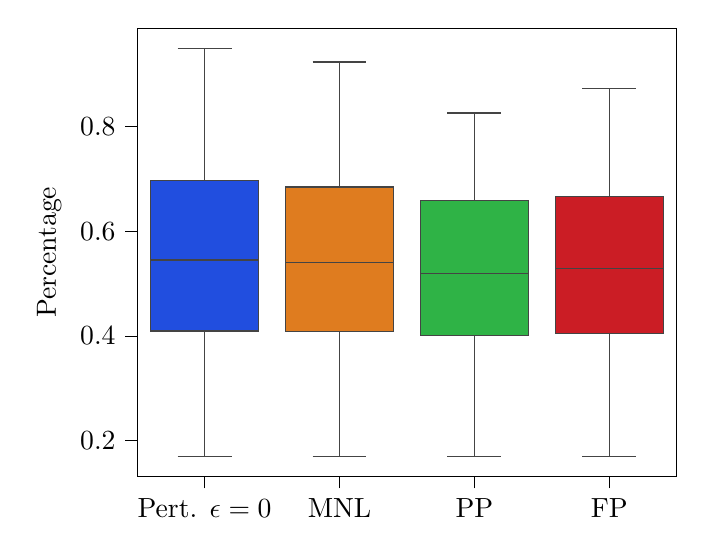
\begin{tikzpicture}

\definecolor{chocolate22312431}{RGB}{223,124,31}
\definecolor{darkgray176}{RGB}{176,176,176}
\definecolor{darkslategray68}{RGB}{68,68,68}
\definecolor{firebrick2032937}{RGB}{203,29,37}
\definecolor{limegreen4717970}{RGB}{47,179,70}
\definecolor{royalblue3378223}{RGB}{33,78,223}

\begin{axis}[
tick align=outside,
tick pos=left,
x grid style={darkgray176},
xmin=-0.5, xmax=3.5,
xtick style={color=black},
xtick={0,1,2,3},
xticklabels={Pert. \(\displaystyle \epsilon=0\),MNL,PP,FP},
y grid style={darkgray176},
ylabel={Percentage},
ymin=0.131064102564103, ymax=0.987653846153846,
ytick style={color=black},
ytick={0,0.2,0.4,0.6,0.8,1},
yticklabels={
  \(\displaystyle {0.0}\),
  \(\displaystyle {0.2}\),
  \(\displaystyle {0.4}\),
  \(\displaystyle {0.6}\),
  \(\displaystyle {0.8}\),
  \(\displaystyle {1.0}\)
}
]
\path [draw=darkslategray68, fill=royalblue3378223]
(axis cs:-0.4,0.409082500924898)
--(axis cs:0.4,0.409082500924898)
--(axis cs:0.4,0.697389063200359)
--(axis cs:-0.4,0.697389063200359)
--(axis cs:-0.4,0.409082500924898)
--cycle;
\addplot [darkslategray68]
table {%
0 0.409082500924898
0 0.17
};
\addplot [darkslategray68]
table {%
0 0.697389063200359
0 0.948717948717949
};
\addplot [darkslategray68]
table {%
-0.2 0.17
0.2 0.17
};
\addplot [darkslategray68]
table {%
-0.2 0.948717948717949
0.2 0.948717948717949
};
\path [draw=darkslategray68, fill=chocolate22312431]
(axis cs:0.6,0.407476686185209)
--(axis cs:1.4,0.407476686185209)
--(axis cs:1.4,0.684222321828776)
--(axis cs:0.6,0.684222321828776)
--(axis cs:0.6,0.407476686185209)
--cycle;
\addplot [darkslategray68]
table {%
1 0.407476686185209
1 0.17
};
\addplot [darkslategray68]
table {%
1 0.684222321828776
1 0.923076923076923
};
\addplot [darkslategray68]
table {%
0.8 0.17
1.2 0.17
};
\addplot [darkslategray68]
table {%
0.8 0.923076923076923
1.2 0.923076923076923
};
\path [draw=darkslategray68, fill=limegreen4717970]
(axis cs:1.6,0.400401214487096)
--(axis cs:2.4,0.400401214487096)
--(axis cs:2.4,0.659233527566114)
--(axis cs:1.6,0.659233527566114)
--(axis cs:1.6,0.400401214487096)
--cycle;
\addplot [darkslategray68]
table {%
2 0.400401214487096
2 0.17
};
\addplot [darkslategray68]
table {%
2 0.659233527566114
2 0.825581395348837
};
\addplot [darkslategray68]
table {%
1.8 0.17
2.2 0.17
};
\addplot [darkslategray68]
table {%
1.8 0.825581395348837
2.2 0.825581395348837
};
\path [draw=darkslategray68, fill=firebrick2032937]
(axis cs:2.6,0.404603122966818)
--(axis cs:3.4,0.404603122966818)
--(axis cs:3.4,0.665313299232737)
--(axis cs:2.6,0.665313299232737)
--(axis cs:2.6,0.404603122966818)
--cycle;
\addplot [darkslategray68]
table {%
3 0.404603122966818
3 0.17
};
\addplot [darkslategray68]
table {%
3 0.665313299232737
3 0.872093023255814
};
\addplot [darkslategray68]
table {%
2.8 0.17
3.2 0.17
};
\addplot [darkslategray68]
table {%
2.8 0.872093023255814
3.2 0.872093023255814
};
\addplot [darkslategray68]
table {%
-0.4 0.544820336391437
0.4 0.544820336391437
};
\addplot [darkslategray68]
table {%
0.6 0.539299242424242
1.4 0.539299242424242
};
\addplot [darkslategray68]
table {%
1.6 0.519677033492823
2.4 0.519677033492823
};
\addplot [darkslategray68]
table {%
2.6 0.527935606060606
3.4 0.527935606060606
};
\end{axis}

\end{tikzpicture}
}}}%
        \caption{\textnormal{Difference in offered compensation from true utility (a) and percentage of utilized gig workers (b) for NYT data (strong preference).}}
        \label{fig:comp_nyt_strong}
    \end{minipage}
\end{figure}

\noindent \textbf{Performance:} Figures \ref{fig:perf_nyt_weak} and \ref{fig:perf_nyt_strong} present boxplots comparing the performance ratios across various benchmarks using weak and strong preference scenarios, respectively. For the weak preference scenario, our algorithm achieves an average performance ratio of 92.6\% (±1.3\%), demonstrating competitive results compared to the Pert. ($\epsilon=0$) benchmark, which attains the highest average performance ratio of 94.0\% (±1.1\%). In comparison, the \gls{acr:pp} benchmark achieves an average performance ratio of 83.0\% (±3.8\%), and the \gls{acr:fp} benchmark yields 84.6\% (±3.0\%). Therefore, our algorithm consistently outperforms the \gls{acr:pp} and \gls{acr:fp} benchmarks. Furthermore, it exhibits low variability and consistent performance, as evidenced by the small standard deviation, and achieves only slightly lower performance than the Pert. ($\epsilon=0$) benchmark. For the strong preference scenario, our algorithm achieves an average performance ratio of 85.3\% (±3.7\%), demonstrating substantial competitiveness, though lower than the Pert. ($\epsilon=0$) benchmark at 91.3\% (±1.6\%). In this scenario, the \gls{acr:pp} and \gls{acr:fp} benchmarks show significantly lower ratios of 60.3\% (±4.2\%) and 65.2\%~(±3.9\%), respectively. Notably, this case shows the greatest relative improvement over benchmark policies among all tested scenarios, highlighting the algorithm's adaptability to more complex preference structures. We attribute the observed gap between our algorithm and the Pert. ($\epsilon=0$) benchmark to challenges in estimating \gls{acr:mnl} parameters under stronger preferences; further refinement in utility estimation could likely enhance performance, aligning the results more closely with the benchmark.
\noindent \textbf{Result 5:} For NYT data, our algorithm achieves performance ratios of 92.6\% for weak and 85.3\% for strong preference scenarios, outperforming rule-based benchmarks by 8–9\% and 20–25\%, respectively.

\noindent \textbf{Compensation and utilized gig workers:} In the following, we examine the offered compensation and the percentage of utilized gig workers. Figures \ref{fig:comp_nyt_weak} and \ref{fig:comp_nyt_strong} display operational metrics for NYT data using gig workers with weak and strong location preferences, respectively. In each figure, part (a) shows the difference between the offered compensation and the deterministic part of the true utility for all accepted requests, while part (b) shows the percentage of utilized gig workers for each policy. We note that the negative values in Figures \ref{fig:comp_nyt_weak}a and \ref{fig:comp_nyt_strong}a are reasonable, as the analysis considers only the deterministic part of the utility, excluding the random component. Consequently, acceptance of requests is still possible if the addition of the stochastic component results in a positive overall utility, which is indeed the case for these observations.  

In the weak preference scenario, the average utilization rate of gig workers remains relatively consistent across all models, at approximately 55\%, with only minor variations of 1–2\%. However, the policies vary in terms of the difference in offered compensation from the true utility. Specifically, the Pert. ($\epsilon=0$) benchmark has a mean difference of only 2.7 monetary units, our algorithm has a mean difference of 3.3 monetary units, and the \gls{acr:pp} and \gls{acr:fp} algorithms have mean differences of 9.8 and 9 monetary units respectively. From these observations, we can conclude that the variation in total reward is mainly due to the lost revenue from offering more compensation than necessary, and not from utilizing a significantly larger amount of gig workers. Therefore, we observe that our algorithm achieves a balance between compensating gig workers and maintaining platform profitability, without the need to overcompensate gig workers to ensure their incentivation.

Considering the strong preference scenario, the average percentage of utilized gig workers is 55\% for the Pert.~($\epsilon=0$) benchmark, 48\% for both our algorithm and the \gls{acr:pp} benchmark, and 46\% for the \gls{acr:fp} benchmark. We observe a reduction in the number of utilized gig workers across all algorithms compared to the Pert.($\epsilon=0$) benchmark. For our algorithm, the lower percentage of utilized gig workers relative to Pert. ($\epsilon=0$) is likely due to an inability to sufficiently incentivize gig workers, particularly for requests where utilities are overestimated, specifically those with dropoff location 1. Despite this, our algorithm demonstrates a similar average difference in offered compensation for accepted requests compared to Pert. ($\epsilon=0$), with mean differences of 2.9 and 3.1 monetary units, respectively. In contrast, the \gls{acr:pp} and \gls{acr:fp} benchmarks show much larger differences of 25.6 and 18.3 monetary units, respectively. This large discrepancy in offered compensation results directly from the benchmarks ignoring gig worker utilities when making decisions.

\noindent \textbf{Result 6:} For the NYT scenario, our algorithm balances compensation and utilization, with mean differences in offered compensation of 3.3 units for weak and 3.1 units for strong preferences, effectively avoiding overcompensation.

\noindent \textbf{Acceptance rates across pickup and dropoff locations}: In the following, we examine the acceptance rates of the various algorithms in handling service requests, based on different pairs of pickup and dropoff locations. We evaluate the algorithms by analyzing the distribution of acceptance probabilities across all location pairs. We employ the Coefficient of Variation (CV) to quantify the balance of acceptance rates of each algorithm. A lower CV signifies a more balanced distribution of acceptance rates across locations. In Figure \ref{fig:fair_nyt_combined}, we observe the percentage of accepted requests and the average utility for each pickup $(p)$ and dropoff $(d)$ location pair $(p,d)$ for weak (Figure \ref{fig:fair_nyt_combined}a) and strong (Figure \ref{fig:fair_nyt_combined}b) location preference scenarios.

\begin{figure}[t]%
    \centering
    \fontsize{10}{10}\selectfont
    \subfloat[\centering NYT with weak location preference gig workers]{\includegraphics[width=0.48\textwidth]{figures/nyt/perc_accepted_and_mean_util.pdf}}%
    \hspace*{0.1cm}
    \subfloat[\centering  NYT with strong location preference gig workers]{\includegraphics[width=0.48\textwidth]{figures/nyt_strong/perc_accepted_and_mean_util.pdf}}%
    \caption{\textnormal{Percentage of accepted requests (white-blue matrix) and average utility (right-side column) for each pickup $(p)$ and dropoff $(d)$ location pair under weak (a) and strong (b) location preferences. Each row represents a different location pair $(p,d)$.}}%
    \label{fig:fair_nyt_combined}%
\end{figure}

For the weak preference scenario, the Pert. ($\epsilon=0$) benchmark and our algorithm exhibit a more equal distribution of acceptance probabilities among all location pairs, with a CV equal to 2.4\% and 2.7\% correspondingly, compared to 5.9\% and 4.4\% for the \gls{acr:pp} and \gls{acr:fp} benchmarks. Even though the \gls{acr:pp} and \gls{acr:fp} benchmarks have a slightly higher CV, the acceptance rates remain relatively balanced among all algorithms. When considering the strong preference scenario, we observe a less balanced distribution of acceptance probabilities  across all algorithms. This indicates a strong influence of location preferences on request acceptance and suggests that strong preferences may lead to certain areas becoming underserved. The Pert. ($\epsilon=0$) benchmark achieves the most balanced distribution, with a CV of 10.3\%. Our algorithm and the \gls{acr:pp} benchmark exhibit similar CVs at 23\% and 23.8\%, respectively, while the \gls{acr:fp} benchmark displays the least balanced distribution, with a CV of 28\%. This result raises potential fairness concerns when using different algorithms, particularly when gig workers exhibit strong preferences for specific request characteristics. Notably, the $(p,d)$ pairs with dropoff location 1 show lower acceptance rates for both our algorithm and the \gls{acr:pp} and \gls{acr:fp} benchmarks. This effect is less pronounced in the Pert. ($\epsilon=0$) benchmark, reinforcing our earlier observation regarding the difficulty in incentivizing gig workers for certain requests. Consequently, we believe that both the percentage of utilized gig workers and the balance of acceptance rates across pickup and dropoff locations can be improved by refining the \gls{acr:mnl} model, ultimately approaching the performance of the Pert. ($\epsilon=0$) benchmark.

\noindent \textbf{Result 7:} For weak location preferences, acceptance rates are consistent across policies (CVs 2.4\%–5.9\%). For strong preferences, Pert. ($\epsilon=0$) achieves the most balanced rates with CV of 10.3\%, while our policy shows a CV of 23\%, comparable to the benchmark policies.
